\chapter{Peak Calling}

The computational method of the protein-chromatin binding event identification plays a central role in ChIP-seq analysis. 
Peak calling is a statistical procedure.
With usage of files having sufficient quality of the mapped IP and control sample, this method produces a BED~\cite{bed} file.
This format represents a set of genomic locations associated with a significance score.

\section{Identification of enriched regions using peak calling}



 
After read mapping to the reference, the next step is to identify loci with high read density comparatively to the background, referred to ChIP-seq signals, or simply peaks.
More than 30 algorithms and tools have been implemented to solve that computational problem~\cite{chen2012systematic}.
The choice of the right peak caller is crucial and depends on the type of experiment~\cite{nakato2017recent}, e.g. TF binding event identification vs. detection of broadly distributed histone marks.

% \todo{to je zavádějící. Nukleosomy sice nevážou konkrétní motiv DNA, ale vykazují jistou míru sekvenčních preferencí, která se liší v závislosti na organismu.}

\begin{figure}[b!]
    \centering
    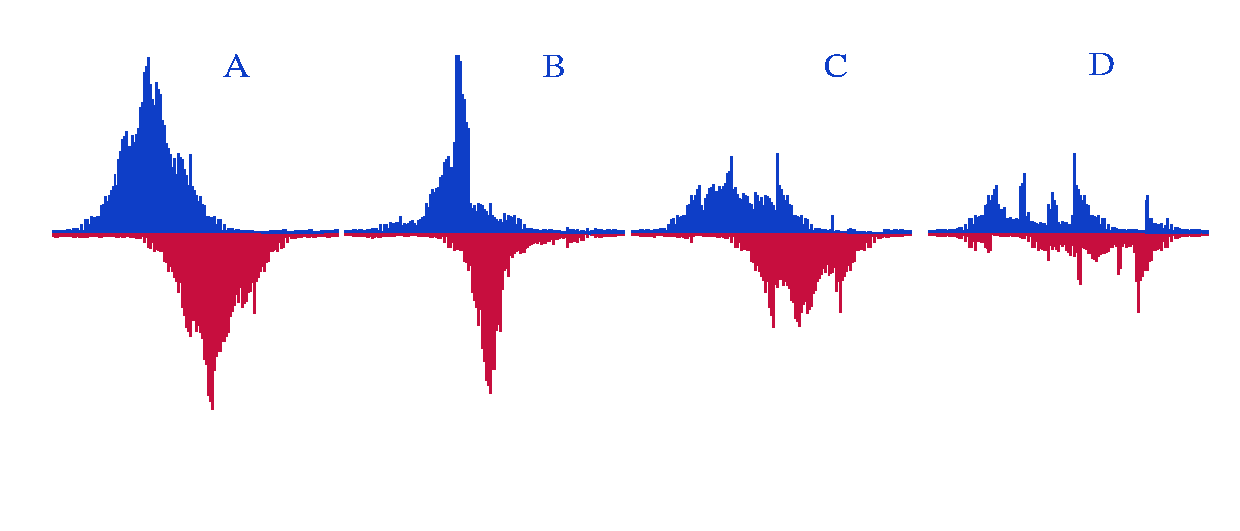
\includegraphics[width=\textwidth]{../img/peaks_final.pdf}
    \caption{Illustration of individual reads mapping to the forward (blue) and reverse (red) strand, building the good bimodal binding site prfile (A, B, C) and false positive (D). }
    \label{peak}
\end{figure}

\paragraph{Peak profile.}
Suitable software builds a peak profile along each chromosome. 
All the peak profiles can be divided into three categories~\cite{park2009chip}. 
Sharp peaks are typical for TF due to dependency on motif sequence~\cite{landt2012chip}. 
Histones have relatively non-specific positioning on the DNA~\cite{krig2007identification}. 
Thus the peak profile is broad and can reach several kilobases. 
The third peak type is a mix of sharp and broad signals, a typical pattern for RNA polymerase II and transcription elongation factor~\cite{squazzo2006suz12, lin2011dynamic}.


The very first extended set methodology to calculate peak profile density was presented in 2007~\cite{robertson2007genome}. 
Fragments are sequenced from $5'$ to $3'$ end, and the minimal required length of a sequenced read is 36 bp. 
But the real fragment of DNA is longer, and thus the interaction of the protein of interest is somewhere on that size-selected longer DNA fragment. 
Each read is computationally extended in the $3'-$ direction. 
Regions are scored by the number of overlapping reads and assessed as a candidate peak.



Sequence directionality sets the stage for a smoothed profile. 
The strand-specific read distributions form a bimodal pattern combined by shifting or extending tags toward the center~\cite{valouev2008genome}.
The example of strand-specific distribution is shown on Figure~\ref{peak}.



\paragraph{Assesment of the candidate regions.}
After scanning through the genome and finding a large number of candidate regions estimating null distribution, the quality of the detected peaks should be determined. 
From generated data, the candidate signal may be either a false or true binding event. 



%And the probabilistic statement cannot be made by using a well known Bayes' Theorem. 
%In the genomic studies, especially in ChIP-seq, individual hypothesis testing is not useful, and a global hypothesis test is required~\cite{futschik2019omnibus}. 

% Suppose we have \textit{n} genomic loci obtained.
% The $i^{th}$ null hypothesis $H_{0,i}$ with corresponding P-values $p_i$.
% The global null hypothesis of simultenious test of all null hypitheses  is defined:

% \begin{align*}
%     H_0 = \displaystyle\bigcap_{i=1}^{n} H_{0, i}
% \end{align*}

% Fisher's combined probability test~\cite{fisher1992statistical} combines known P-values:

% \begin{align*}
%     T = - \displaystyle \sum_{i=1}^{n} 2 \log p_i \sim  \chi_{2n}^{2}
% \end{align*}

% Bonferroni's test~\cite{hommel1988stagewise} looks at the smallest P-value and at given desired level $\alpha$ tests the global null hypothesis by testing each $H_{0,i}$ at level $\alpha /n$. 
% And whenever $p_i \leq \alpha / n$ rejects the global null hypothesis.
% Assuming the global hypothesis is true, the overal level control is: 

% \begin{align*}
%     P_{H_0}[Error Type I] = P_{H_0} \left[\bigcup_{i=1}^{n} \left\{ p_i \leq \alpha / n\right\}\right] \leq \sum_{i=1}^{n} P_{H_0}(p_i \le \alpha / n)  = n \frac{\alpha}{n} = \alpha
% \end{align*}

% %\todo{pro Fishera a FWER chybí citace}
% Even though both tests are easy and straightforward, non of them is effective. 
% Fisher's test will be eliminated in a large number of the true null hypothesis. 
% In the case of  Bonferroni's test, the only one P-value is used. 
% Hence it can be applied only if very few binding events are expected to be significant. 
% The rejection of extreme value of binding event at the $\alpha$ significance level leads to increase number of false positives. 
% The idea of the global null hypothesis rejection is not suitable for genomic analysis. 
% Another approach is the familywise error rate (FWER)~\cite{lehmann2012generalizations} method:

% \begin{align*}
%     FWER \leq 1 - (1 - \alpha)^c, 
% \end{align*}

% where $\alpha$ is a level for an individual test, $c$ is a number of comparisons.
% The test controls the probability of performing one or more Type I errors. 
% However, the method is very conservative and does only a few rejections. 
% FWER is closely related to the false discovery rate (FDR), which in fact increases statistical power  and makes fewer false positives. 
% The application of FDR approach in the genomic field was first associated with microarray technology~\cite{lai2017statistical}.

% %The method allows a few small rejections if the majority of the rejections are correct. 
% %\todo{nerozumím, co znamená "SMALL rejection"}
% %Such testing adjusts the statistical confidence based on the number of tests. 

% Let $R$ be the total number of rejections and $V$ be the number of trully null hypotheses.
% The the proportion $Q$ of false positive rejection among all rejection is 

% \begin{align*}
%     Q = \frac{V}{R} .
% \end{align*}

% The Benjamini-Hochberg procedure~\cite{benjamini2000adaptive} ensures the expectetion and define False Dicovery Rate as follow: 

% \begin{align*}
%     FDR = E(Q) = E \left(\frac{V}{R}\right) .
% \end{align*}

% If all null hypotheses are true, then FDR and FWER are indeed the same.
% The most common significance level accepted is 95, which means that 95\% of the obtained result has a chance to be true. 
% The p = 0,05 cutoff means that the chance of making a wrong decision is equal to 5\%. 
% It is too strict and leads to the loss of a real finding. 
% That is why the q-value was introduced to calibrate the false discovery rate measurements~\cite{storey2003statistical}. 
% P-value test the significance of the false-positive rates and the q-value test the significance in term of false discovery rate. 
% In other words, the threshold choice either by P- or q-value should be based on how many false positives are expected in the experiment.


%\section{Statistical Model Utilization for the Assesment of the Significance of Estimated Signals.}

Standard biological research has some rate of false positives. 
Due to that there is no absolute proof or absolute rejection of the results in ChIP-seq studies, the analysis works with probabilities.
The end goal of the ChIP-seq experiment is to define the genomic loci of possible protein binding events. 
The null hypothesis $H_{0}$ is the default assumption for the model generating the data; the alternative hypothesis $H_{A}$ is accepted as the best explanation for the data if the $H_{0}$ is rejected.
The candidate signal of a binding event is represented as an alternative hypothesis $H_{A}$, and $H_{0}$ is that there is no actual binding. 
To describe the statistical significance of the individual hypothesis, a $p$-value is calculated.

Different scientific studies based on statistical approaches utilize either $p$-value or confidence intervals concepts. 
Even though those two concepts are complementary, many biological and medical studies prefer confidence intervals to $p$-value because of showing the potential range of results~\cite{feinstein1998p}.
However, there are several reasons why the utilization of the $p$-value in the ChIP-seq studies is more suitable than confidence intervals.


The early approach was to assume that the background noise is uniform; 
However, the usage of the control dataset shows that the different biases make the uniform model too ideal to be true~\cite{robertson2007genome}. 
That is why all peak calling algorithms make all the output signals associated with $p$-value~\cite{chitpin2019recap} to determine statistical significance in a hypothesis test. 
The incorrect rejection on the null hypothesis produces the Type-I error known as a ``false positive''. 
In the context of ChIP-seq analysis, this type of error occurs when there is no actual binding event, but the peak caller shows that there is. 
The inversion of Type-I error is Type-II error, which is referred to as a ``false negative''. 
Considering the common clinical experiments, the ``false negative'' error type is seen as less serious than the ``false positive'' error.
However, in ChIP-seq experiment, the false positives can be checked by qPCR experiment, whereas the ``false negatives'' are going to be lost. 

In~\ref{pvalue} and~\ref{qvalue} we give an explanation of basic statistics used for peak evaluation in more detail.

% To test peaks for significance, different peak calling algorithms adopt different statistical techniques. 
% In a MUSIC's approach~\cite{harmanci2014music}, a window of fixed size for TF or varying width for histone marks while scanning a genome ranks the candidate peaks using a Binomial test.

% % \begin{align*}
% %     p_{k,n} = \binom{n}{k}p^k(1-p)^{n-k}
% % \end{align*}

% The widely used Poisson model was utilized in early software tools such as SICER~\cite{zang2009clustering}. 
% The Poisson is directly connected to Binomial distribution,
% where probability \textit{p} of succes in each trail and p$_{k,n}$  for \textit{k} succes in \textit{n} trails; but assosiated with rare events:

% % \begin{align*}
% %     p_{0,n} = (1 - p)^{n} = \left(1-{\frac{\lambda}{n}}\right)^{n} \to e^{-\lambda}
% % \end{align*}

% % \begin{align*}
% %     p_{1,n} = np(1 - p)^{n-1} = \frac{\lambda}{1-p}\left(1-{\frac{\lambda}{n}}\right)^{n} \to \lambda e^{-\lambda}
% % \end{align*}

% % \begin{align*}
% %     p_{2,n} = \frac{1}{2} n(n - 1) p^{2} (1-p)^{n-2} = \frac{1}{2} \frac{\lambda^{2} - \lambda p}{ (1-p)^{2}} \left(1-{\frac{\lambda}{n}}\right)^{n} \to \frac{1}{2} \lambda^{2} e^{-\lambda}
% % \end{align*}

% For \textit{k} succes in \textit{n} trails with probability p=${\lambda / n}$ , the binomial probability p$_{n,k}$ approaches the Poisson probability:

% \begin{align*}
%     P_k = \frac{\lambda _i ^{k}}{k!} e^{- \lambda _i}
% \end{align*}

% The Poisson parameter $\lambda_i$ is supposed to be constant across the genome and provided to be inadequate for ChIP-seq peak calling to identify TFs binding sites. 
% The negative binomial model was suggested by CisGenome~\cite{ji2008inte}, which is, in fact, a generalization of the Poisson distribution, also known as the gamma-Poisson mixture distribution. 

% \begin{align*}
%     NB_{y_i; \mu _i, \alpha} = \frac{\Gamma (y_i + \alpha ^{-1})}{\Gamma(\alpha ^{-1})\Gamma(y_i + 1)} \left(\frac{\alpha ^{-1}}{\alpha ^{-1} + \mu_i}\right) ^{\alpha ^{-1}} \left(\frac{ \mu _i}{ \alpha ^{-1} + \mu _i}\right) ^{y _i}
% \end{align*}

% The derevation from two-parameter gamma distribution is done in on page 118 in~\cite[Cameron and Trivedi (2013)]{cameron2013regression}.

% Another suggestion was to estimate $\lambda$ for each genomic position by the local Poisson test. 
% Such an approach was introduced by the most popular peak caller called MACS~\cite{zhang2008model}.
% The tool slides with a constant size window centered on each nucleotide across the genome, merge overlapping peaks by extending the read.
% If the number of reads in the IP sample is higher than expected, given a background rate estimated from the control dataset, then using the Poison test, the enriched regions are ranked~\cite{thomas2017features}. 
% The highest tag pileup is defined as a summit of a signal.  

% Comparing the statistical models implemented by different peak calling algorithms shows that the Poisson test is a better approach to score the candidate signals than the Binomial test~\cite{thomas2017features}.




\section{Introduction into Hypothesis Testing}
\label{pvalue}
In this section, we give a light introduction into hypothesis testing, from the point of view of classical statistics.
It is a very important part of statistcs, often used in biological research.
In this whole part, we loosely follow~\cite{bertsekas2002introduction}.

In general, hypotheses are assumptions or statements about parameters of probability distributions.
% Examples include the fowllowing:
% \begin{itemize}
% \item
% A coin is biased.
% \item
% The avarage grade of a student is $2.5$.
% \item
% The avarage delivery time of the post is at least $2$ days.
% \item
% People spend more time on social media during the weekends.
% \end{itemize}
These statements can be either true or false.
Further, we can distighuish several types of hypotheses:
\begin{itemize}
\item
Simple: the parameter takes one specific value. %, e.g., \emph{``The probability of falling heads is $2/3$''}.
\item
Composite: the parameter takes one specific value. %, e.g., \emph{``The probability of falling heads is $1/3$ or $2/3$''}.
\item
One-sided: the parameter is on one side of some specific value. %, e.g., \emph{``The expected time of package delivery is $\leq 10$ days''}.
\item
Two-sided: the parameter is on two sides of some specific value. %, e.g., \emph{``The probability of falling heads is not $2/3$''}
\end{itemize}

\paragraph{Null and alternative hypotheses.}
The status quo, or our belief, is typically represented by the \emph{null hypothesis}, denoted by $H_0$.
The complementary view is represented by the \emph{alternative hypothesis}, usually denoted by $H_A$, or also by $H_1$.
The alternative hypothesis can be for example the complement, or the ``one-sided'' complement of $H_0$.

% \begin{example}
% For a two-sided coin a possible null hypothesis is the following:
% $$H_0: \quad\text{the coin is unbiased, i.e., $P(\text{heads}) = 1/2$.}$$
% The complementary hypothesis is:
% $$H_A: \quad\text{$P(\text{heads}) \neq 1/2$.}$$
% A possible one-sided alternative is:
% $$H_A: \quad\text{$P(\text{heads}) > 1/2$.}$$
% \qed
% \end{example}

\paragraph{Testing.}
In classical statistics, testing hypothesis is performed in several steps.
First, we designs an experiment.
Next, it is necessary to collect the data.
Finally, we check whether the date is consistent with the null hypothesis $H_0$.

If indeed the date is consistent with $H_0$, then we \emph{do not reject the null hypothesis $H_0$}.
On the other hand, if the data is inconsistent with the null hypothesis $H_0$, we \emph{reject $H_0$ in favor of the alternative hypothesis $H_A$}.

Equivalently, we could say that we do reject $H_0$ if there is a strong evidence towards the alternative, and we do not reject $H_0$ if there is not a strong evindence towards the alternative.

In the following $P_{H_0}$ denotes the probability under the assumption that $H_0$ is true.
Slightly more formally, the whole process could be summarized as follows:
\begin{itemize}
\item
Define a numerical outcome $X$ of the experiment, called the \emph{test statistic}.
More precisely, $T$ is some function of the data related to the experiment.
\item
Determine the distribution of $X$ under the hypothesis $H_0$, i.e., determine the probabilities $P_{H_0}(X=x)$, for all possible values of $x$.
\item
Determine the value $x$ of $X$ for the observed data.
\item
Look at the probability $P_{H_0}(x)$.
If it is large, then we say that the data is consistent with $H_0$ and we do not reject $H_0$.
If it is small, then we reject $H_0$ in favor of $H_A$.
\end{itemize}
Note that we give the words ``large'' and ``small'' a more precise meaning later, when we discuss error types.

% \begin{example}
% Consider the hypotheses $H_0: \text{the coin is unbiased}$, and a one sided alternative $H_A: \text{the coin is biased with $P(\text{heads}) > 1/2$}$.
% In a possible experiment, we could toss the coin, say, $20$ times.
% The test statistic could be a function of the data that counts the number of heads $X$ in those $20$ tosses.
% We could could say that if $X \geq 16$, then $H_0$ is unlikely and we might reject $H_0$ towards $H_A$.
% \qed
% \end{example}

\begin{remark}
It is important to note the asymmetry between the null hypothesis and alternative hypothesis.
The null hypothesis can be rejected towards the alternative, thus confirming the alternative.
The other option is that we \emph{do not reject} the null hypothesis, which means that our data are no inconsistent with the null.
This does not mean that we confirm the null hypothesis.
\end{remark}

\paragraph{Types of errors.}
There are in general two types of errors.
\begin{itemize}
\item
\emph{Type-I error (false positive):} we reject the null hypothesis even though it is true.
\item
\emph{Type-II error (false negative):}  we do not reject null hypothesis even though it is not true.
\end{itemize}
Usually the type-I error is much more significant and we describe two possible methods to deal with them.

Recall that we want to reject the null hypothesis only if there is strong eveidence for the alternative.
To make this statement more precise using probability, let $\alpha$ be some small constant, called \emph{significance level} (typically $0,01$ or $0.05$).
Now, we say that if $H_0$ is true, then accept $H_A$ with probability at most $\alpha$, i.e.,
$$P_{H_0}(\text{accept $H_A$}) \leq \alpha.$$
This exactly means that we want the probability of type-I error to be small.
We recall two methods to achieve this: \emph{critical-value} and \emph{$p$-value}.

\paragraph{Critical-value.}
For give significance level $\alpha$ the \emph{critical-value} $x_\alpha$ is a threshold such that such that if the numerical outcome of the experiment is greater or equal than $x_\alpha$, we accept $H_A$, and, otherwise, we do not reject $H_0$.
The number $x_\alpha$ depends on $\alpha$, and recall that $\alpha$ is an upper bound for the probability of type-I error.
So, if we make $\alpha$ very small, we will accept $H_A$ only for large values.

To find $x_\alpha$, it suffices to note that by definition
$$P_{H_0}(X\geq x_\alpha) = P_{H_0}(\text{falsely accept $H_A$}) \leq \alpha.$$
Thus, we need
$$P_{H_0}(X\geq x_\alpha) \leq \alpha.$$
However, if we set $x_\alpha$ unnecessarily large, we will amost never accept $H_A$.
Therefore, we look for the smallest $x$ such that $P_{H_0}(X \geq x) \leq \alpha$ and set this to be the cirtical-value $x_\alpha$.


\paragraph{$p$-value.}
Instead of finding the critical-values, one can directly work with the distribution $X$, which is the motivation for $p$-values.
Notice that for a cricital value $x_\alpha$, we accept $H_A$ if and only if $x\geq x_\alpha$.
This is equivalent to
$$P_{H_0}(X\geq x) \leq P_{H_0}(X\geq x_\alpha)\leq\alpha.$$
Similarly, we do not reject $H_0$ if an only if $x < x_\alpha$, which is equivalent to
$$P_{H_0}(X\geq x) > \alpha.$$
This, we can define the \emph{$p$-value} of $x$ to be just the probability $P_{H_0}(X\geq x)$.
This gives us the same regions for $H_0$ and $H_A$ without knowing $x_\alpha$, which can be hard to compute for some distributions.

Let us summarize what we obtained.
For a significance level $\alpha$ and an outcome of the experiment $x$, it suffices to it suffices to look at the probability $P_{H_0}(X\geq x)$.
If $P_{H_0}(X\geq x) \geq \alpha$, we can accept $H_A$, otherwise we do not reject $H_0$.



\section{Multiple hypothesis testing}
\label{qvalue}

In this section, we continue with a light introduction to multiple hypothesis testing, false discovery rate (FDR), and $q$-value.
The term $q$-value was defined originally in~\cite{storey2003positive} in order to controll the false discovery rate in multiple hypothesis testing.
In this section, we follow this paper.

As mentioned in the previous section, when testing one hypothesis, we are typically concerend with controlling the false positive rate.
In other words, we are maximizing the power while keeping the Type-I error rate below some level.
In the field of multiple hypothesis testing this basic paradigm is extended to the situation where several hypothesis are tested simultaneously.
The challenge is to define an appropriate measure of false psitives one is willing to encounter.

\paragraph{FWER.}
Until 90's the most common measure for testing multiple hypothesis is \emph{family wise error rate} (FWER), which is defined to be the probability of getting one or more false positives out of all tested hypotheses, i.e., $$\text{FWER} := P(V \geq 1),$$ where $V$ is the number of false positives.
For example, if $\alpha$ is a significance level (as in the previous section) and there are $m$ hypotheses tested, then each test is controlled so that the probability of getting a false positive is less than or equal to $\alpha/m$.
Clearly, then the overall FWER is less than or equal to $\alpha$.
This method is called Bonferroni's method and other methods can be found, for example, in~\cite{shaffer1994multiple}.

In some instances of multiple hypothesis testing, one might be more concerned about the rate of false positives among all rejected hypotheses rather than the probability of making some Type-I errors.
In this regard FWER gives a very strict cirterion, which is not always appropriate.
In other words, FWER is conservative in order to avoid false positives at the cost of being less powerfull, i.e., it has lower probability of rejecting the null hypothesis correctly.

\paragraph{FDR.}
In a seminal paper, Benjamini and Hochberg introduced introduced an error measure for multiple hypothesis testing called the \emph{false dicovery rate} (FDR). To define this, we will first need to fix some notation.

Suppose we have $m$ null hypotheses, denoted by $H_1,\dots, H_m$.
As described in the previous section, using a statistical test, we reject the null hypotheses if the test is declared significant, otherwise we do not reject it.
By taking the sum of each type of outcome over all $H_i$, we get the following important random variables:
\begin{itemize}
\item
$V$, the number of false positives (also called Type-I error or false discoveries),
\item
$S$, the number of true positives (also called true discoveries),
\item
$T$, the number of false negatives (also called Type-II error),
\item
$U$, the number of true negatives,
\item
$R = V + S$, the number of rejected null hypotheses (also called discoveries, true or false).
\end{itemize}
Let $m_0$ be the number of true null hypotheses.
Out of $m$ hypothesis tests, $R$ is a random variable that we can actually observe and the other random variables $S$, $T$, $U$ and $V$ are unobservable.
The whole situation can be summarized in the following table:

\begin{center}
\begin{tabular}[h]{|l|c|c|c|}
\hline
& Null  is true & Alternative is true & Total\\
\hline
Null is rejected & $V$ & $S$ & $R$\\
\hline
Null is not rejected  & $U$ & $T$ & $m - R$\\
\hline
Total  & $m_0$ & $m - m_0$ & $m$\\
\hline
\end{tabular}
\end{center}

Benjamini and Hochberg (1995)~\cite{benjamini1995controlling}, defined the false discovery rate by
$$\text{FDR} := E(V/R \mid R > 0) \cdot P(R > 0),$$
where $E(\cdot)$ denotes the expected value.
To explain this formula, it is worth noting that we are really interested in the expected value of the ratio $V/R$, and the use of the conditional expectation is just a technicallity to avoid division by zero.
Thus, $\text{FDR}$ is the expected proportion of the false discoveries among the discoveries (rejections of the null hypothesis).
The goal is to keep $\text{FDR}$ below some treshold.


Benjamini and Hochberg also proposed a procedure for controlling $\text{FDR}$ and it can be briefly described as follows.
For the $m$ hypothesis tests we obtain $p$-values $p_1,\dots,p_m$ and without loss of generality we may assume that $p_1 \leq \cdots \leq p_m$.
Benjamini and Hochberg caculate the quantity
$$k' := \underset{1\leq k\leq m}{\text{arg\,max}}\{k : p_k \leq \alpha \cdot k/m\},$$
where $\alpha$ is the significance level.
Now, rejecting null hypotheses corresponding to the $p$-values $p_1,\dots,p_{k'}$ results in
$$\text{FDR} = m_0/m \cdot \alpha \leq \alpha.$$
Note that, the definition of $\text{FDR}$ uses expected value, and therefore it is not guaranteed that for any set of data $V/R \leq \alpha$.
The expected value tells us only that the long term long-term behaviour (expected) of this procedure gives $\text{FDR} \leq \alpha$.
The $\text{FDR}$ is less conservative and in many situations it is arguably more appropriate approach thatn $\text{FWER}$.
This implies that $\text{FDR}$ has more power, i.e., a higher probability of correctly rejecting the null hypotheses, at the cost of increased number of false positives.

\paragraph{pFDR.}
The \emph{positive false discovery rate} (pFDR) is a modified version of FDR, originally introduced in~\cite{storey2003positive}.
The author motivates the concept as follows.
Probably, the most obvious definition of FDR would be just the expected value $E(V/R)$, however, this is not well-defined if $R=0$.
Then, as already mentioned, the formula in the definition of $\text{FDR}$ is one possible quantity that can fix this problem.
Another possible quantity would be the positive false discovery rate, defined by
$$\text{pFDR} := E(V/R \mid R > 0).$$

\paragraph{$q$-value.}
In~\cite{storey2003positive}, the \emph{$q$-value} was introduced as the pFDR analogue of the $p$-value.
It gives a hypothesis testing error measure for each observed statistic with respect to the pFDR.

To introduce the $q$-value, we need some new notation.
For a given significance level $\alpha$, let $\Gamma_\alpha$ be the region on the real line where null hypothesis is rejected, i.e.,
$$P_{H_0}(T \in \Gamma_\alpha) = \alpha,$$
where $T$ is the test statistic of the observed data.
If $\alpha' \leq \alpha$, we have $\Gamma_{\alpha'} \subseteq \Gamma_\alpha$.
A reformulation of the definition of the $p$-value of an observed statistic $T = t$ from the previous section is
$$\text{$p$-value}(t) := \inf_{\{\Gamma_\alpha : t \in \Gamma_\alpha\}}\{P_{H_0}(T \in \Gamma_\alpha)\},$$
where $\inf\{\cdot\}$ denotes the infimum of a set.

The $q$-value is is defined for an observed statistic $T = t$ in an analogous way.
Namely,
$$\text{$q$-value}(t) := \inf_{\{\Gamma_\alpha : t \in \Gamma_\alpha\}}\text{pFDR}(\Gamma_\alpha).$$
Thus, the $q$-value is the infimum of the $\text{pFDR}$ if $H_0$ is rejected for test statistics with values greater or equal than $t$.
Equivalently, the $q$-value is the infimum of the probability that $H_0$ is true given that $H_0$ is rejected (the false discovery rate).

A possible interpretation is the following: the proportion of the false positives among all positive results.
For a set of test statistics and their $q$-values, rejecting the null hypothesis for all tests $q$-value is less than or equal to some $\alpha$ ensures that the expected value of the false discovery rate is $\alpha$.







%%%%%%%%%%%%%%%%%%%%%%%%%%%%%%%%%%%%%%%%%%%%%
\section{Statistical Sin and Reliability of the Obtained List of ChIP-seq Signals After Peak Calling Procedure}

Most programs for identification of the enriched regions (peaks) work as follow: candidate signal are identified by analyzing along the genome, and then by comparing with the input or mock dataset(or with another IP data in case of the differential analysis) regions are evaluated. 
However, most of the software tools use data twice to identify and assess the enrichment, which leads to a statistical sin~\cite{lun2014novo}. 
Moreover, the estimated $p$-values depend on the same data and result in statistical bias.
A similar problem can influence the result during ChIP-seq analysis and in areas such as DNA variant calling~\cite{chitpin2019recap}.

Without a correctly calculated $p$-value, it is difficult to choose the right cutoff, which influences the final results. 
Improper $p$-values lead to difficulties in evaluating of reliability of a given set of peaks.
It may also lead to loss of a true binding event due to the biased statistical significance of such a peak, and further downstream analysis will exhibit an error-prone result~\cite{chitpin2019recap}. 

\paragraph{Solutions.}
A possible solution to that problem is to develop a new peak identification approach to avoid double usage of the same data. 
However, many software tools are good enough to be used, and recalibration of the obtained $p$-values is a possible alternative resolve~\cite{chitpin2019recap}.


Peak identification process outputs typically tens of thousands of possible binding loci, which are needed to be assessed. 
An obtained list of peak coordinates may be annotated with the nearest gene. 
However, the lack of annotated actual binding sites may limit the process of the validation of the experiment result~\cite{nakato2017recent}.

The motif-discovery of a peak collection is another available approach. 
Typically the top-$p$-value-ranked peaks are undergoing the motif finding procedure~\cite{bailey2011dreme}.
Motifs are represented as a position weight matrix and sequence logo and suitable for the TF experiment due to the specificity of the binding protein.
However, for the proteins which bind without a preferable sequence such as histones, the motif-based evaluation of the peak reliability is not suitable~\cite{nakato2017recent}. 

If more than one biological replicates are available, then another way to validate signals is to assess the global similarity between replicates with a calculation of the cross-correlation coefficient. 
IDR, which validates the rank consistency of common peaks in replicates, is another way for the peak validation, which may help to filter out false-positive peaks. 

As  was mentioned, the bimodal peak pattern is utilized in peak calling design. 
Many false positives may be filtered out by analyzing the size and appearance of the signal~\cite{rye2011manually}. 
However, only a few methods utilize the analysis of the peak shapes~\cite{hower2011shape, wu2014polyapeak}.
